\subsection{Vue d'ensemble de \touist}\label{sec:sat_interface}

\touist est composé de trois modules, mais l'utilisateur standard ne verra que l'un d'entre eux : l'interface. Dans la suite nous insistons principalement sur cette dernière plutôt que sur le traducteur et le solveur. L'architecture globale est illustrée par la figure~\ref{fig:architectureTouisT}:

\begin{figure}[htbp]
\centering
% 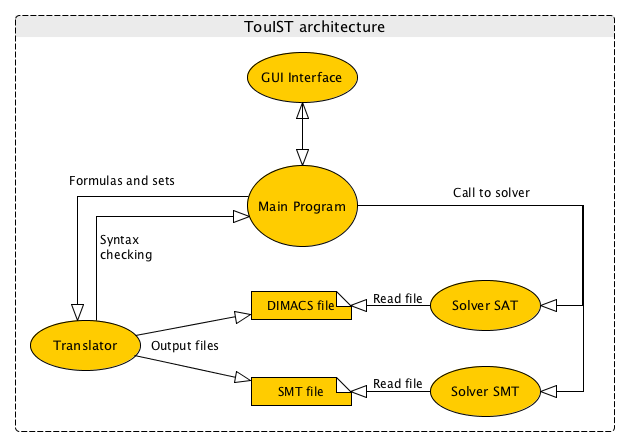
\includegraphics[scale=0.37]{figures/DiagTouist.png}
  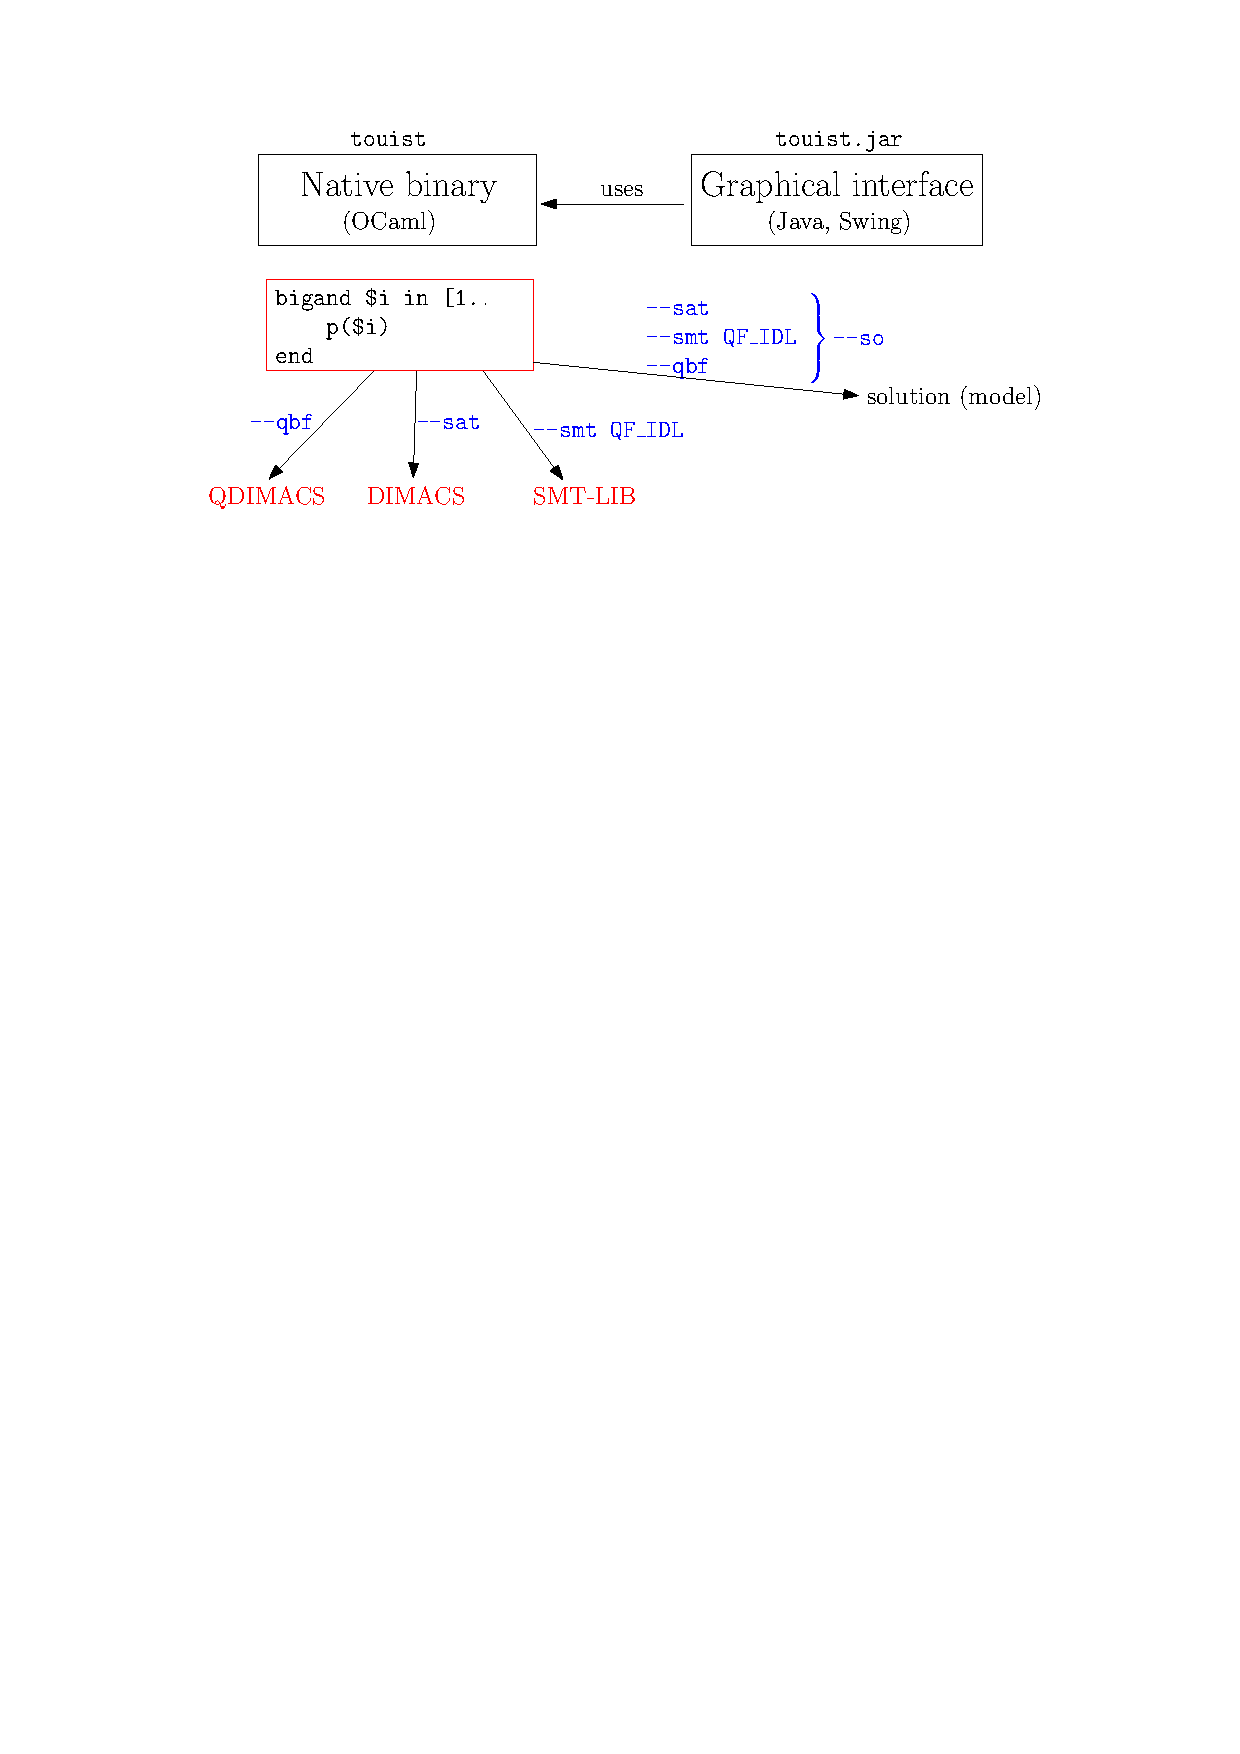
\includegraphics[scale=0.80]{figures/architecture.pdf}
  \caption{Architecture de TouIST}
  \label{fig:architectureTouisT}
\end{figure}

Avec \touist , on accède à un éditeur puissant et convivial pour éditer des formules logiques complexes et des contraintes variées comme :

\[\bigwedge_{i \in \{1..9\}} (P_i \IMPL Q_{i+1})\]

\noindent
qui s'écrira simplement en \touist :
% bash ./scripts/touist-to-latex-et-verbatim.sh <<< 'bigand $i in [1..9]: P(i) => Q(i+1) end'
\begin{mdpre}%mdk
\noindent{\mdcolor{navy}bigand}~{\mdcolor{purple}\$i}~{\mdcolor{navy}in}~{}[{\mdcolor{purple}1}..{\mdcolor{purple}9}]:\\
~~~~P(i)~=\textgreater{}~Q(i+{\mdcolor{purple}1})\\
{\mdcolor{navy}end}%mdk
\end{mdpre}%mdk

\noindent
qui abrège confortablement :\\

\[(P_1 \Rightarrow Q_2) \AND (P_2 \IMPL Q_3) \AND \ldots (P_9\IMPL Q_{10}).\] 
\\

%%%%%%%%%%%%%%%%%%%%%%%%%%%%%%%

Une fois qu'une formule a été donnée à l'interface, sa satisfiabilité peut être vérifiée : l'interface peut l'envoyer au prouveur qui retourne un modèle, affiché comme le montre la figure \ref{fig:capture-modeles} si un tel modèle existe. Ensuite, par l'intermédiaire de l'interface, l'utilisateur peut par exemple demander d'autres modèles (bouton \enquote{Next} de l'interface). Contrairement à \satoulouse qui aurait nécessité de modifier les formules pour interdire le modèle et de relancer le solveur, \touist conserve une instance du solveur en attente, ce qui permet d'obtenir les modèles suivants bien plus rapidement.

Les modèles renvoyés par le solveur sont totaux : une valeur est affectée à chacune des variables apparaissant dans les formules envoyées au solveur. L'utilisateur peut sélectionner uniquement les propositions vraies ou les propositions fausses. Il peut également sélectionner des sous-ensembles de variables en tapant une expression régulière pour les filtrer.


%%%%%%%%%%%%%%%%
- l'éditeur de langage \touist
- le prouveur (solveur)

mais aussi

- la traduction vers des langages compatibles avec les solveur
- la traduction vers \LaTeX

mais encore

- un éditeur web en cours de développement
- touist (command line) est dispo sur OPAM et sur Homebrew (dans un tap)

Parler aussi du langage touist qui recoupe
- la logique prop
- SMT
- QBF
- et meme DLPA
\begin{figure}
  \centering
  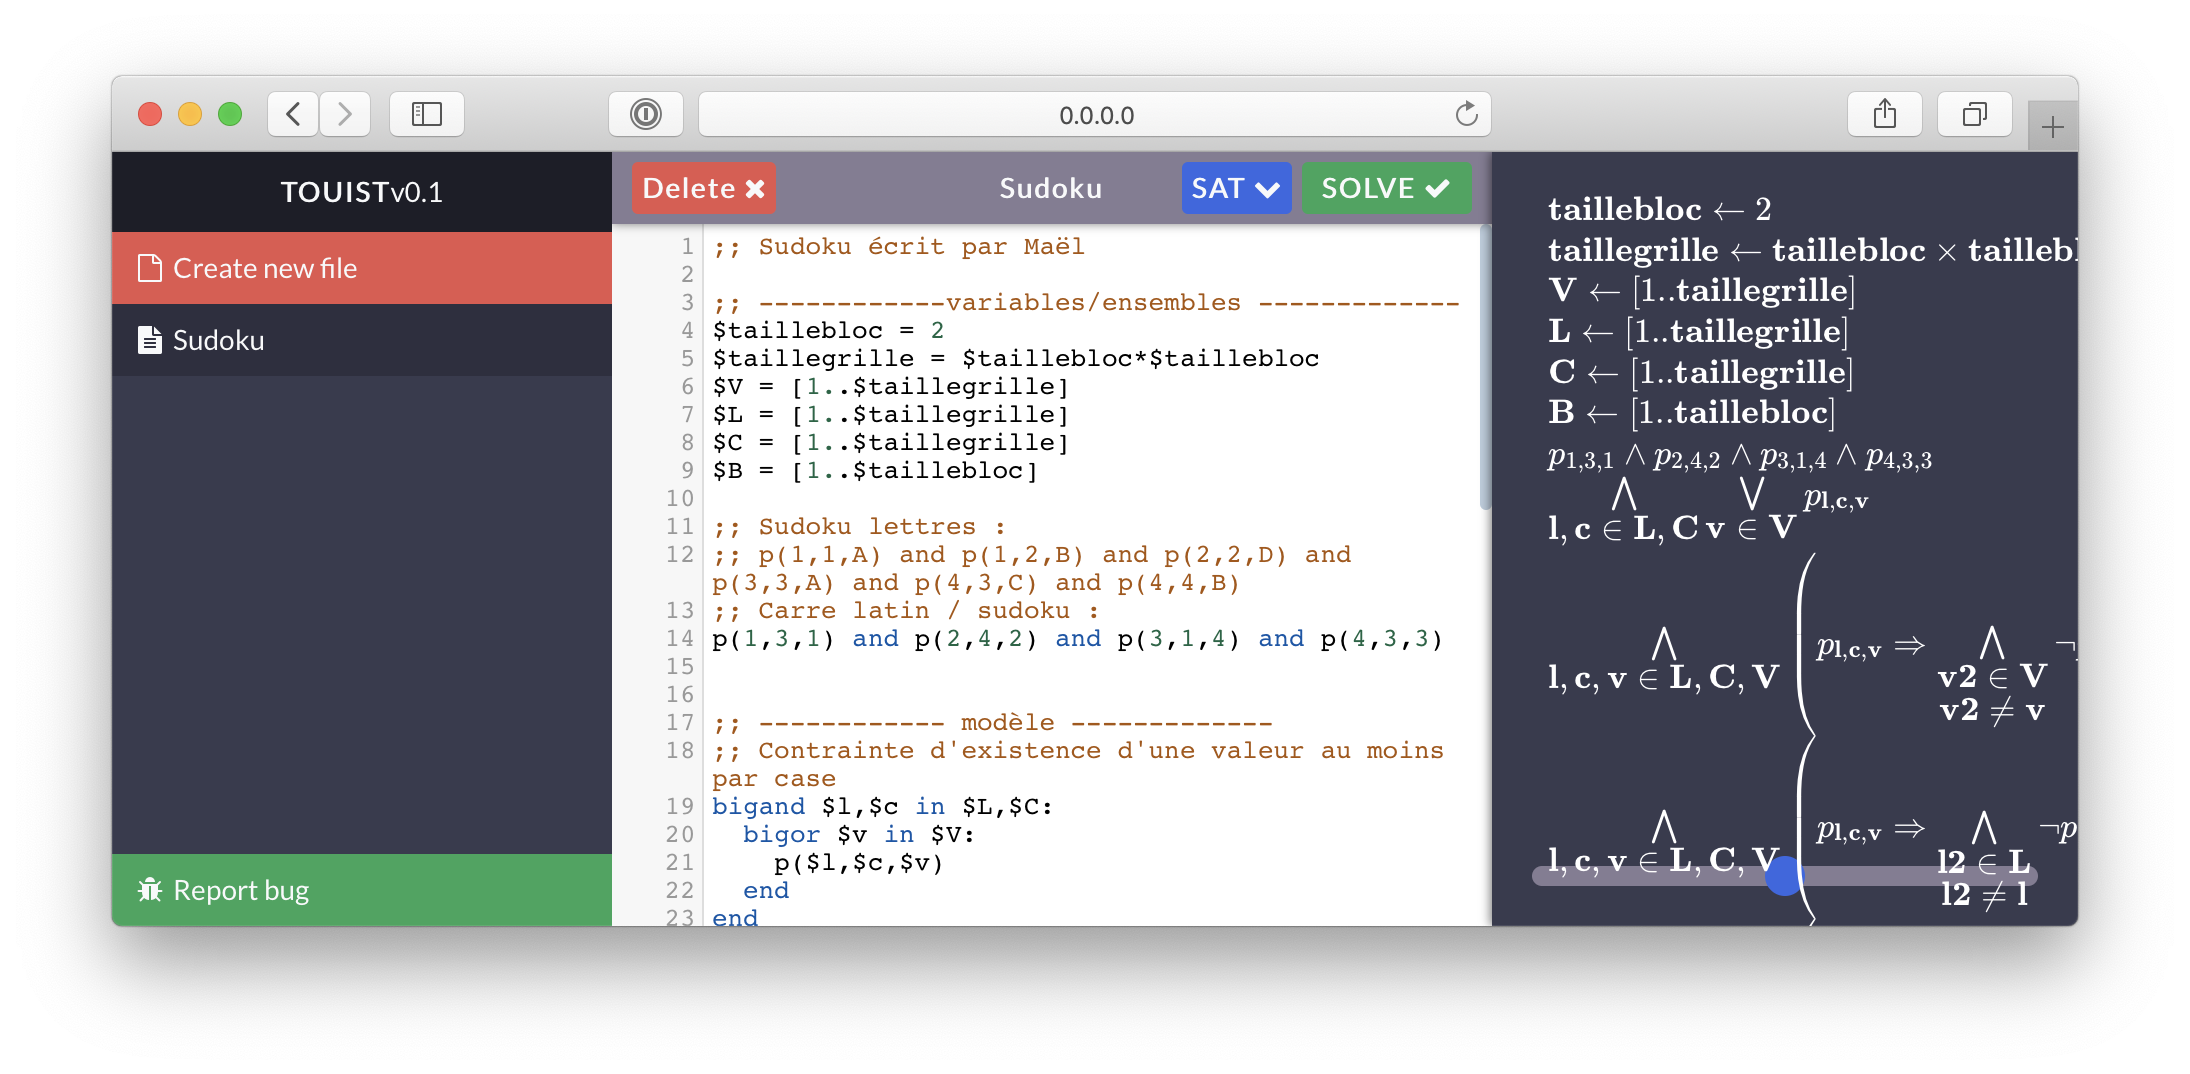
\includegraphics[scale=0.80]{figures/touist-web}
  \caption{Architecture de \touist}
  \label{fig:architectureTouisT}
\end{figure}